\documentclass[
    10pt,
    oneside,
    a4paper,
    %english,
    italian
]{book}

\PassOptionsToPackage{dvipsnames}{xcolor} % colori PDF/A

\usepackage{colorprofiles}
% PDF/A
% validate in https://www.pdf-online.com/osa/validate.aspx
\usepackage[a-1a,mathxmp]{pdfx}[2018/12/22]
%\usepackage{amsmath,amssymb,amsthm} % matematica
\usepackage[T1]{fontenc}
\usepackage[utf8]{inputenc}
\usepackage[italian]{babel}
\usepackage{bookmark}
\usepackage{caption}
\usepackage{chngpage, calc} % centra il frontespizio
\usepackage{csquotes} % gestisce automaticamente i caratteri (")
\usepackage{emptypage} % pagine vuote senza testatina e piede di pagina
\usepackage{epigraph} % per epigrafi
%\usepackage{indentfirst} % rientra il primo paragrafo di ogni sezione
\usepackage{graphicx} % immagini
\usepackage[pdfa]{hyperref} % collegamenti ipertestuali
%\usepackage{hyperref}
\usepackage{listings} % codici
%\usepackage{microtype} % microtipografia
\usepackage{mparhack,relsize}  % finezze tipografiche
\usepackage{nameref} % visualizza nome dei riferimenti
\usepackage[font=small]{quoting} % citazioni
\usepackage{subfig} % sottofigure, sottotabelle
\usepackage[italian]{varioref} % riferimenti completi della pagina
\usepackage{booktabs} % tabelle
\usepackage{tabularx} % tabelle di larghezza prefissata
\usepackage{longtable} % tabelle su più pagine
\usepackage{ltxtable} % tabelle su più pagine e adattabili in larghezza
\usepackage[toc, acronym, automake]{glossaries}
\usepackage[backend=biber,style=verbose-ibid,hyperref,backref]{biblatex}
%\usepackage{layaureo} % margini ottimizzati per l'A4
\usepackage{lmodern}
\usepackage[left = 1in + 17pt + 0.6cm]{geometry} % Increased margins for single-page printing
\usepackage[inkscapelatex=false]{svg}
\usepackage{fancyhdr}
\usepackage{lipsum}
\usepackage{setspace}
\usepackage{titlesec}
% Load variables
\newcommand{\myUni}{Università degli Studi di Padova}
\newcommand{\myDepartment}{Dipartimento di Matematica ``Tullio Levi-Civita''}
\newcommand{\myFaculty}{Corso di Laurea in Informatica}
\newcommand{\myTitle}{Lorem ipsum dolor sit amet, consectetur adipisci elit.}
\newcommand{\myDegree}{Tesi di Laurea} % Rimossa la voce "Triennale" poichè "Tesi di Laurea" già sottintende la laurea triennale, in quanto è il titolo accademico base
\newcommand{\profTitle}{Prof.}
\newcommand{\myProf}{Cognome Nome}
\newcommand{\graduateTitle}{Laureando}
\newcommand{\myName}{Paolino Paperino}
\newcommand{\myStudentID}{1234567}
\newcommand{\myAA}{20XX-20XX}
\newcommand{\myLocation}{Padova}
\newcommand{\myTime}{Mese 20XX}
% Acronyms
\newacronym[description={\glslink{apig}{Application Programming Interface}}]
    {api}{API}{Application Program Interface}

\newacronym[description={\glslink{sdkg}{Software Development Kit}}]
    {sdk}{SDK}{Software Development Kit}

\newacronym[description={\glslink{umlg}{Unified Modeling Language}}]
    {uml}{UML}{Unified Modeling Language}

% Glossary entries
\newglossaryentry{apig} {
    name=\glslink{apig}{API}
    text=Application Program Interface,
    sort=api,
    description={In informatica con il termine \emph{API} si indica ogni insieme di procedure disponibili al programmatore, di solito raggruppate a formare un set di strumenti specifici per l'espletamento di un determinato compito all'interno di un certo programma. La finalità è ottenere un'astrazione, di solito tra l'hardware e il programmatore o tra software a basso e quello ad alto livello semplificando così il lavoro di programmazione}
}

\newglossaryentry{sdkg} {
    name=\glslink{sdkg}{SDK}
    text=SDK,
    sort=sdk,
    description={A software development kit (SDK) is a collection of software development tools in one installable package. They facilitate the creation of applications by having a compiler, debugger and sometimes a software framework. They are normally specific to a hardware platform and operating system combination. To create applications with advanced functionalities such as advertisements, push notifications, etc; most application software developers use specific software development kits}
}

\newglossaryentry{umlg} {
    name=\glslink{umlg}{UML}
    text=UML,
    sort=uml,
    description={In ingegneria del software \emph{Unified Modeling Language} (ing. linguaggio di modellazione unificato) è un linguaggio di modellazione e specifica basato sul paradigma object-oriented. L'\emph{UML} svolge un'importantissima funzione di ``lingua franca'' nella comunità della progettazione e programmazione a oggetti. Gran parte della letteratura di settore usa tale linguaggio per descrivere soluzioni analitiche e progettuali in modo sintetico e comprensibile a un vasto pubblico}
}


%\newglossaryentry{qiskitg} {
    %name=\glslink{qiskit}{Qiskit},
    %text=Qiskit,
    %sort=qiskit,
    %description={Qiskit ([quiss-kit] noun, software) %is an open-source SDK for working with quantum %computers at the level of extended quantum %circuits, operators, and primitives.}
%}

\makeglossaries

\glsaddall

\bibliography{appendix/bibliography}

\defbibheading{bibliography} {
    \cleardoublepage
    \phantomsection
    \addcontentsline{toc}{chapter}{\bibname}
    \chapter*{\bibname\markboth{\bibname}{\bibname}}
}

%Improvements the paragraph command
\titleformat{\paragraph}
{\normalfont\normalsize\bfseries}{\theparagraph}{1em}{}
\titlespacing*{\paragraph}
{0pt}{3.25ex plus 1ex minus .2ex}{1.5ex plus .2ex}

% Custom hyphenation rules
\hyphenation {
    e-sem-pio
    ex-am-ple
}

% Images path
\graphicspath{{img/}}

% Force page color, as some editors set a grayish color as default
\pagecolor{white}

%Define custom colors
% \definecolor{lavenderindigo}{rgb}{0.58, 0.34, 0.92}
\definecolor{hyperColor}{HTML}{0041EB}

\captionsetup{
    tableposition=top,
    figureposition=bottom,
    font=small,
    format=hang,
    labelfont=bf
}

\hypersetup{
    %hyperfootnotes=false,
    %pdfpagelabels,
    colorlinks=true,
    linktocpage=true,
    pdfstartpage=1,
    pdfstartview=,
    breaklinks=true,
    pdfpagemode=UseNone,
    pageanchor=true,
    pdfpagemode=UseOutlines,
    plainpages=false,
    bookmarksnumbered,
    bookmarksopen=true,
    bookmarksopenlevel=1,
    hypertexnames=true,
    pdfhighlight=/O,
    %nesting=true,
    %frenchlinks,
    %urlcolor=lavenderindigo,
    %linkcolor=blue,
    %citecolor=webgreen,
    %pagecolor=blue,
    allcolors = hyperColor,
}

% Delete all links and show them in black, useful for printing
% \hypersetup{draft}

% Listings setup
\lstset{
    language=[LaTeX]Tex,%C++,
    keywordstyle=\color{RoyalBlue}, %\bfseries,
    basicstyle=\small\ttfamily,
    %identifierstyle=\color{NavyBlue},
    commentstyle=\color{Green}\ttfamily,
    stringstyle=\rmfamily,
    numbers=none, %left,%
    numberstyle=\scriptsize, %\tiny
    stepnumber=5,
    numbersep=8pt,
    showstringspaces=false,
    breaklines=true,
    frameround=ftff,
    frame=single
}

\newcommand{\sectionname}{sezione}
\addto\captionsitalian{\renewcommand{\figurename}{Figura}
                       \renewcommand{\tablename}{Tabella}}

\newcommand{\glsfirstoccur}{\ap{{[g]}}}

\newcommand{\intro}[1]{\emph{\textsf{#1}}}

% Risks environment
\newcounter{riskcounter} % define a counter
\setcounter{riskcounter}{0} % set the counter to some initial value
%%%% Parameters
% #1: Title
\newenvironment{risk}[1]{
    \refstepcounter{riskcounter} % increment counter
    \par \noindent % start new paragraph
    \textbf{\arabic{riskcounter}. #1} % display the title before the content of the environment is displayed
}{
    \par\medskip
}

\newcommand{\riskname}{Rischio}
\newcommand{\riskdescription}[1]{\textbf{\\Descrizione:} #1.}
\newcommand{\risksolution}[1]{\textbf{\\Soluzione:} #1.}

% Use case environment
\newcounter{usecasecounter} % define a counter
\setcounter{usecasecounter}{0} % set the counter to some initial value

%%%% Parameters
% #1: ID
% #2: Nome
\newenvironment{usecase}[2]{
    \renewcommand{\theusecasecounter}{\usecasename #1}  % this is where the display of the counter is overwritten/modified
    \refstepcounter{usecasecounter} % increment counter
    \vspace{10pt}
    \par \noindent % start new paragraph
    {\large \textbf{\usecasename #1: #2}} % display the title before the content of the environment is displayed
    \medskip
}{
    \medskip
}
\newcommand{\usecasename}{UC}
\newcommand{\usecaseactors}[1]{\textbf{\\Attori Principali:} #1. \vspace{4pt}}
\newcommand{\usecasepre}[1]{\textbf{\\Precondizioni:} #1. \vspace{4pt}}
\newcommand{\usecasedesc}[1]{\textbf{\\Descrizione:} #1. \vspace{4pt}}
\newcommand{\usecasepost}[1]{\textbf{\\Postcondizioni:} #1. \vspace{4pt}}
\newcommand{\usecasealt}[1]{\textbf{\\Scenario Alternativo:} #1. \vspace{4pt}}

% Namespace description environment
\newenvironment{namespacedesc}{
    \vspace{10pt}
    \par \noindent  % start new paragraph
    \begin{description}
}{
    \end{description}
    \medskip
}

\newcommand{\classdesc}[2]{\item[\textbf{#1:}] #2}

%\linespread{1.25}
\setstretch{1.5}

%\hypersetup{pdfstartview=} commentato il 9/11/23

\newcommand{\textbfit}[1]{\textbf{\textit{#1}}}

\pagestyle{fancy}
\fancyhf{}
\fancyhead[L]{\leftmark}
% \fancyhead[R]{\thepage} %For plading the page numer on the top right
\fancyfoot[C]{\thepage} %For plading the page numer on the bottom of the page

\date{}

\hypersetup{pdfstartview=}
\begin{document}
    %\layout
    
    \frontmatter
    \begin{titlepage}
    \begin{center}
        \begin{LARGE}
            \textbf{\myUni}\\
        \end{LARGE}

        \vspace{5pt}

        \begin{Large}
            \textsc{\myDepartment}\\
        \end{Large}

        \vspace{5pt}

        \begin{large}
            \textsc{\myFaculty}\\
        \end{large}

        \vspace{25pt}
        
        \begin{figure}[htbp]
            \centering
            
\includegraphics[height=6cm]{img/logo_unipd.jpeg}
        \end{figure}
        
        \vspace{25pt}

        \begin{LARGE}
            \textbf{\myTitle}\\
        \end{LARGE}

        \vspace{10pt}

        \begin{large}
            \textsl{\myDegree}\\
        \end{large}

        \vspace{46pt}
        
        \begin{large}
            \begin{flushleft}
                \textit{Relatore}\\
                \vspace{3pt}
                \profTitle\ \myProf
            \end{flushleft}

            \vspace{-37pt}
            
            \begin{flushright}
                \textit{Laureando}\\
                \vspace{3pt}
                \myName\\
                \vspace{3pt}
                Matricola \myStudentID
            \end{flushright}
        \end{large}

        \vspace*{\fill}
        
        \line(1, 0){338} \\
        \begin{normalsize}
            \textsc{Anno Accademico \myAA}
        \end{normalsize}
    \end{center}
\end{titlepage}

    \clearpage
\phantomsection
\thispagestyle{empty}
\hfill
\vfill

{\small\noindent\textcopyright\ \myName, \myTime. Tutti i diritti riservati. \myDegree: ``\textit{\myTitle}'', \myUni, \myDepartment, \myFaculty.}
    \input{preface/3_acknowledgements}
    \input{preface/4_abstract}
    \input{preface/5_table_of_contents}

    \backmatter
    \printglossary[type=\acronymtype, title=Acronimi e abbreviazioni, toctitle=Acronimi e abbreviazioni]
    \printglossary[type=main, title=Glossario, toctitle=Glossario]
    
    \cleardoublepage

    \mainmatter
    \chapter{Introduzione}
\label{cap:introduzione}

\begin{figure}[h!]
    \centering
    
\includegraphics[width=1\columnwidth]{img/quantum_entanglement.jpeg}
    \caption{Lorem}
    \label{fig:entanglement}
\end{figure}

Introduzione al contesto applicativo.

Lorem Figure \ref{fig:entanglement}

Esempio di utilizzo di un termine nel glossario \gls{api}.

Esempio di citazione in linea
\cite{site:agile-manifesto}.

Esempio di citazione nel pie' di pagina
citazione\footcite{womak:lean-thinking}

Termine di glossario \gls{apig}

\lipsum[1-2]

\section{L'azienda}

\lipsum[1]

\section{L'idea}

Introduzione all'idea dello stage\footcite{article:spooky}.
\lipsum[1-3]

\section{Organizzazione del testo}

\begin{description}
    \item[{\hyperref[cap:processi-metodologie]{Il secondo capitolo}}] descrive ...
    
    \item[{\hyperref[cap:descrizione-stage]{Il terzo capitolo}}] approfondisce ...
    
    \item[{\hyperref[cap:analisi-requisiti]{Il quarto capitolo}}] approfondisce ...
    
    \item[{\hyperref[cap:progettazione-codifica]{Il quinto capitolo}}] approfondisce ...
    
    \item[{\hyperref[cap:verifica-validazione]{Il sesto capitolo}}] approfondisce ...
    
    \item[{\hyperref[cap:conclusioni]{Nel settimo capitolo}}] descrive ...
\end{description}

Riguardo la stesura del testo, relativamente al documento sono state adottate le seguenti convenzioni tipografiche:
\begin{itemize}
	\item gli acronimi, le abbreviazioni e i termini ambigui o di uso non comune menzionati vengono definiti nel glossario, situato alla fine del presente documento;
	%\item per la prima occorrenza dei termini riportati nel glossario viene utilizzata la seguente nomenclatura: \emph{parola}\glsfirstoccur;
	\item i termini in lingua straniera o facenti parti del gergo tecnico sono evidenziati con il carattere \emph{corsivo}.
\end{itemize}

    \chapter{Processi e metodologie}
\label{cap:processi-metodologie}

Lorem ipsum dolor sit amet, consectetuer adipiscing elit. Aenean commodo ligula eget dolor. Aenean massa. Cum sociis natoque penatibus et magnis dis parturient montes, nascetur ridiculus mus. Donec quam felis, ultricies nec, pellentesque eu, pretium quis, sem.

\cite{article:spooky}

\begin{figure}[h]
    \centering
    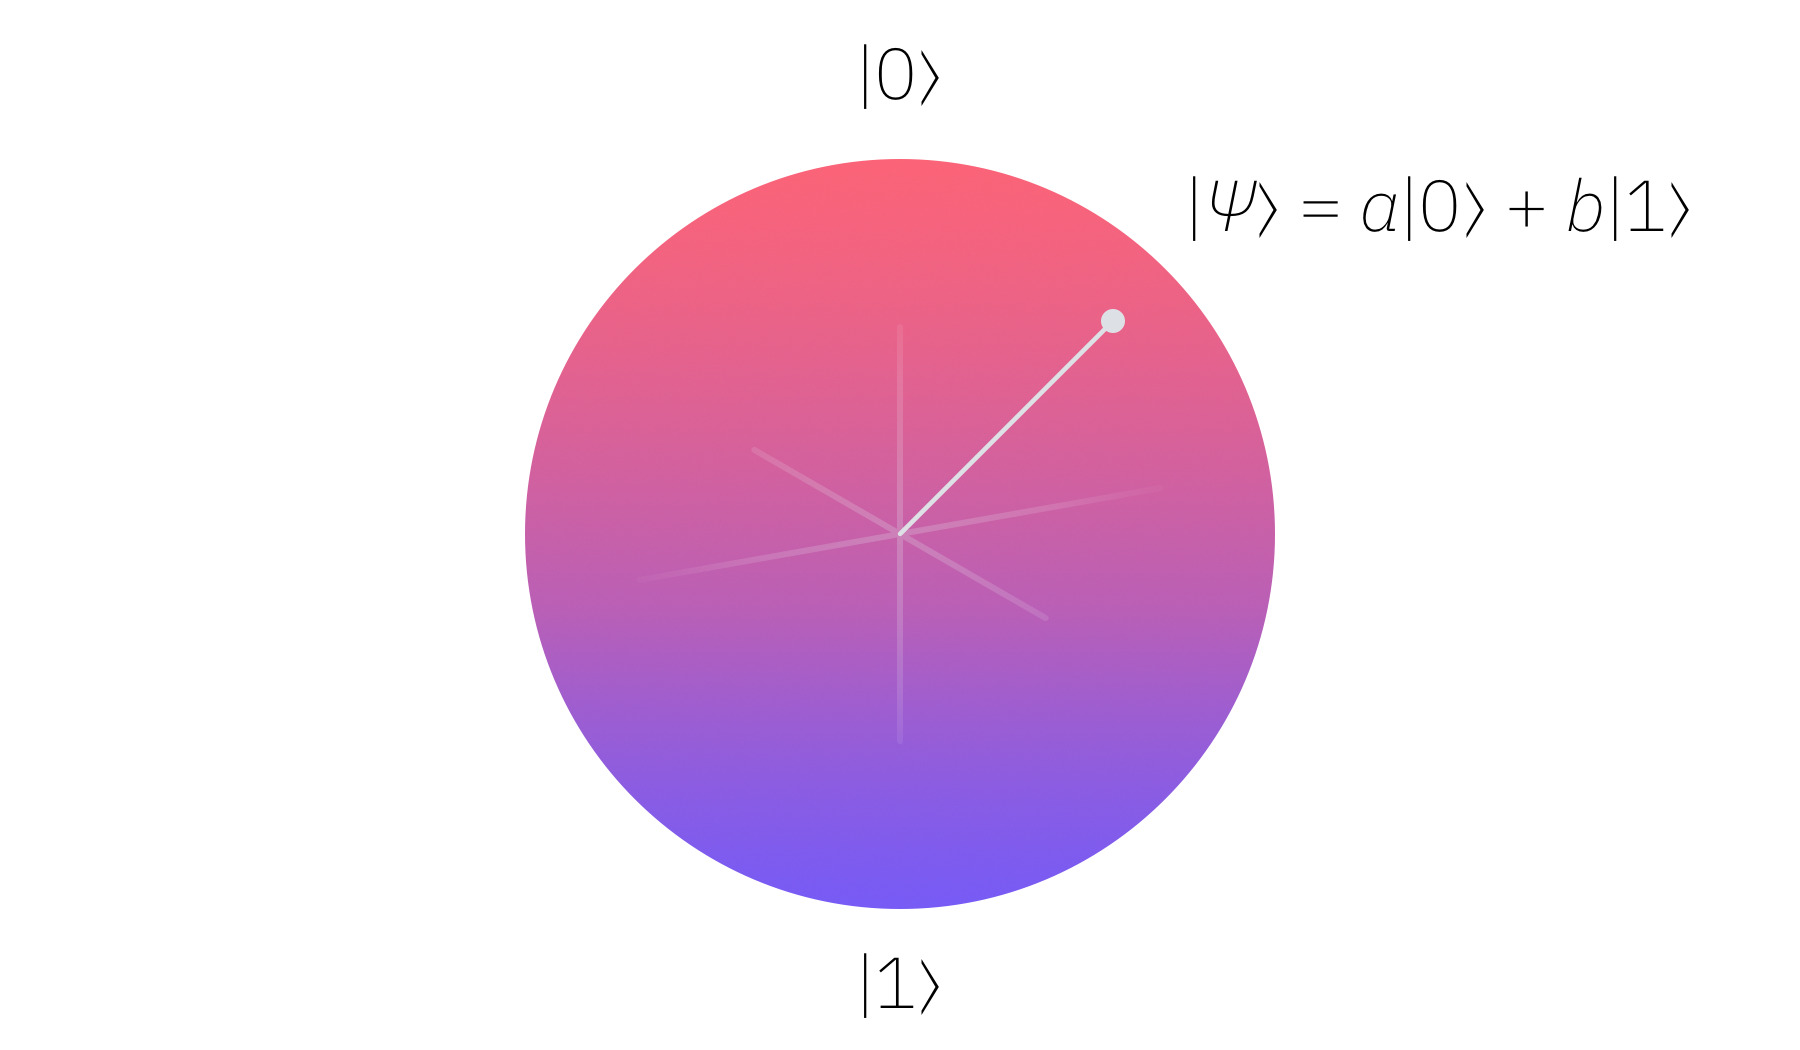
\includegraphics[height=5cm]{img/qubit.jpeg}
    \caption{Lorem}
    \label{fig:qubit}
\end{figure}

\lipsum[1]

\section{Processo sviluppo prodotto}

    \chapter{Descrizione dello stage}
\label{chap:descrizione-stage}

%\intro{Breve introduzione al capitolo}\\

\section{Introduzione al progetto}

\begin{figure}[!ht] 
    \centering 
    
\includegraphics[width=0.5\columnwidth]{pk_estate.jpeg} 
    \caption{Caption}
    \label{fig:pk_estate}
\end{figure}
\lipsum[1]

\section{Analisi preventiva dei rischi}

Durante la fase di analisi iniziale sono stati individuati alcuni possibili rischi a cui si potrà andare incontro.
Si è quindi proceduto a elaborare delle possibili soluzioni per far fronte a tali rischi.

\begin{risk}{Performance del simulatore hardware}
    \riskdescription{le performance del simulatore hardware e la comunicazione con questo potrebbero risultare lenti o non abbastanza buoni da causare il fallimento dei test}
    \risksolution{coinvolgimento del responsabile a capo del progetto relativo il simulatore hardware}
    \label{risk:hardware-simulator} 
\end{risk}

\section{Requisiti e obiettivi}

\section{Pianificazione}
Lorem

\subsection{Ipsum}
Dolor

\subsubsection{Sit}
Amet

\paragraph{Memento}
mori
    % chktex-file 8
% chktex-file 44
% chktex-file 24
\chapter{Analisi dei requisiti}
\label{cap:analisi-requisiti}

\section{Casi d'uso}

Per lo studio dei casi di utilizzo del prodotto sono stati creati dei diagrammi.
I diagrammi dei casi d'uso (in inglese \emph{Use Case Diagram}) sono diagrammi di tipo \gls{uml} dedicati alla descrizione delle funzioni o servizi offerti da un sistema, così come sono percepiti e utilizzati dagli attori che interagiscono col sistema stesso.
Essendo il progetto finalizzato alla creazione di un tool per l'automazione di un processo, le interazioni da parte dell'utilizzatore devono essere ovviamente ridotte allo stretto necessario. Per questo motivo i diagrammi d'uso risultano semplici e in numero ridotto.

\begin{figure}[ht] 
    \centering 
    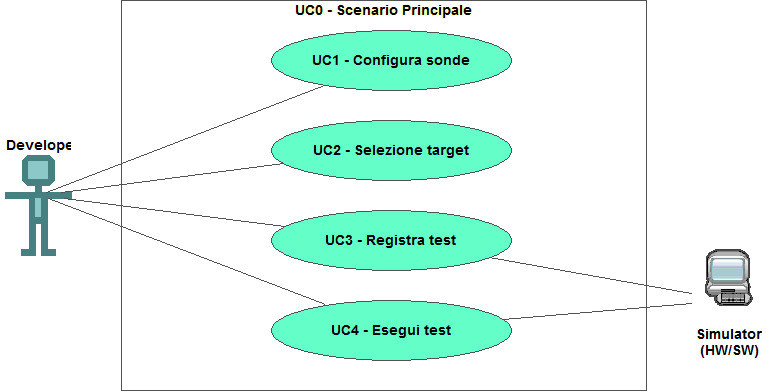
\includegraphics[width=0.7\columnwidth]{usecase/scenario-principale} 
    \caption{Use Case - UC0: Scenario principale}
\end{figure}

\begin{usecase}{0}{Scenario principale}
    \usecaseactors{Sviluppatore applicativi}
    \usecasepre{Lo sviluppatore è entrato nel plug-in di simulazione all'interno dell'IDE}
    \usecasedesc{La finestra di simulazione mette a disposizione i comandi per configurare, registrare o eseguire un test}
    \usecasepost{Il sistema è pronto per permettere una nuova interazione}
\label{uc:scenario-principale}
\end{usecase}

\section{Casi d'uso}
\begin{usecase}{1}{Gestione Utente}
    \usecaseactors{Amministratore, Utente Registrato}
    \usecasepre{L'utente deve essere autenticato nel sistema.}
    \usecasedesc{L'utente può gestire le informazioni del proprio profilo.}
    \usecasepost{Le modifiche vengono salvate nel sistema.}
    \usecasealt{Se l'utente non è autenticato, visualizza un messaggio di errore.}
\end{usecase}

\begin{usecase}{2}{Creazione Prodotto}
    \usecaseactors{Amministratore}
    \usecasepre{L'amministratore ha effettuato l'accesso al sistema.}
    \usecasedesc{L'amministratore può aggiungere un nuovo prodotto al catalogo.}
    \usecasepost{Il nuovo prodotto viene aggiunto con successo.}
    \usecasealt{Se i campi obbligatori non sono compilati, visualizza un messaggio di errore.}
\end{usecase}

\section{Tracciamento dei requisiti}

Da un'attenta analisi dei requisiti e degli use case effettuata sul progetto è stata stilata la tabella che traccia i requisiti in rapporto agli use case.\\
Sono stati individuati diversi tipi di requisiti e si è quindi fatto utilizzo di un codice identificativo per distinguerli.\\
Il codice dei requisiti, dove ogni requisito è identificato con il carattere \textbf{R}, è così strutturato:

\begin{enumerate}
    \item[\textbf{F}:] Funzionale.
    \item[\textbf{Q}:] Qualitativo.
    \item[\textbf{V}:] Di vincolo.
    \item[\textbf{N}:] Obbligatorio (necessario).
    \item[\textbf{D}:] Desiderabile.
    \item[\textbf{Z}:] Opzionale.
\end{enumerate}

Nelle tabelle \ref{tab:requisiti-funzionali}, \ref{tab:requisiti-qualitativi} e \ref{tab:requisiti-vincolo} sono riassunti i requisiti e il loro tracciamento con gli use case delineati in fase di analisi.

\section{Tabelle dei requisiti}

\begin{table}[h]
\begin{tabularx}{\textwidth}{lXl}
\hline
    \textbf{Requisito} & \textbf{Descrizione} & \textbf{Use Case}\\
    \hline
    RFN-1 & L'interfaccia permette di configurare il tipo di sonde del test & UC1\\
\hline
\end{tabularx}
\vspace{4pt}
\caption{Tabella del tracciamento dei requisti funzionali}
\label{tab:requisiti-funzionali}
\end{table}

\begin{table}[h]
\begin{tabularx}{\textwidth}{lXl}
\hline
    \textbf{Requisito} & \textbf{Descrizione} & \textbf{Use Case}\\
    \hline
    RQD-1    & Le prestazioni del simulatore hardware deve garantire la giusta esecuzione dei test e non la generazione di falsi negativi & - \\
\hline
\end{tabularx}
\vspace{4pt}
\caption{Tabella del tracciamento dei requisiti qualitativi}
\label{tab:requisiti-qualitativi}
\end{table}

\begin{table}[h]
\begin{tabularx}{\textwidth}{lXl}
\hline
    \textbf{Requisito} & \textbf{Descrizione} & \textbf{Use Case}\\
    \hline
    RVO-1    & La libreria per l'esecuzione dei test automatici deve essere riutilizzabile & - \\
\hline
\end{tabularx}
\vspace{4pt}
\caption{Tabella del tracciamento dei requisiti di vincolo}
\label{tab:requisiti-vincolo}
\end{table}
    \chapter{Progettazione e codifica}
\label{chap:progettazione-codifica}

Breve introduzione al capitolo

\section{Tecnologie e strumenti}
\label{sec:tecnologie-strumenti}

Di seguito viene data una panoramica delle tecnologie e strumenti utilizzati.

\subsection*{Tecnologia 1}
Descrizione Tecnologia 1.

\subsection*{Tecnologia 2}
Descrizione Tecnologia 2

\section{Ciclo di vita del software}
\label{sec:ciclo-vita-software}

\section{Progettazione}
\label{sec:progettazione}

\subsection{Namespace 1} %**************************
Descrizione namespace 1.

\begin{namespacedesc}
    \classdesc{Classe 1}{Descrizione classe 1}
    \classdesc{Classe 2}{Descrizione classe 2}
\end{namespacedesc}


\section{Design Pattern utilizzati}

\section{Codifica}

    \chapter{Verifica e validazione}
\label{chap:verifica-validazione}

\begin{figure}[h!]
    \centering
    
\includegraphics[width=1\columnwidth]{img/quantum_superposition.jpeg}
    \caption{Lorem}
    \label{fig:enter-label}
\end{figure}

\lipsum[1-2]
    \chapter{Conclusioni}
\label{cap:conclusioni}
Lorem

% per avere termine di glossario con apice "g" che appare
Lorem \glsfirstoccur{\gls{sdkg}}\\
% per avere termine di glossario normale
Lorem \gls{apig}


\section{Consuntivo finale}

Ipsum

\section{Raggiungimento degli obiettivi}

Sit amet



\section{Conoscenze acquisite}

\section{Valutazione personale}


    \appendix
    \backmatter
    \chapter{Bibliografia}
\label{chap:bibliography}

\nocite{*}

% Books bibliography
\printbibliography[heading=subbibliography, title={Books}, type=book]

% Articles bibliography
\printbibliography[heading=subbibliography, title={Articles}, type=article]

% Websites bibliography
\printbibliography[heading=subbibliography, title={Websites}, type=online]

    % Acronyms
\newacronym[description={\glslink{apig}{Application Programming Interface}}]
    {api}{API}{Application Program Interface}

\newacronym[description={\glslink{sdkg}{Software Development Kit}}]
    {sdk}{SDK}{Software Development Kit}

\newacronym[description={\glslink{umlg}{Unified Modeling Language}}]
    {uml}{UML}{Unified Modeling Language}

% Glossary entries
\newglossaryentry{apig} {
    name=\glslink{apig}{API}
    text=Application Program Interface,
    sort=api,
    description={In informatica con il termine \emph{API} si indica ogni insieme di procedure disponibili al programmatore, di solito raggruppate a formare un set di strumenti specifici per l'espletamento di un determinato compito all'interno di un certo programma. La finalità è ottenere un'astrazione, di solito tra l'hardware e il programmatore o tra software a basso e quello ad alto livello semplificando così il lavoro di programmazione}
}

\newglossaryentry{sdkg} {
    name=\glslink{sdkg}{SDK}
    text=SDK,
    sort=sdk,
    description={A software development kit (SDK) is a collection of software development tools in one installable package. They facilitate the creation of applications by having a compiler, debugger and sometimes a software framework. They are normally specific to a hardware platform and operating system combination. To create applications with advanced functionalities such as advertisements, push notifications, etc; most application software developers use specific software development kits}
}

\newglossaryentry{umlg} {
    name=\glslink{umlg}{UML}
    text=UML,
    sort=uml,
    description={In ingegneria del software \emph{Unified Modeling Language} (ing. linguaggio di modellazione unificato) è un linguaggio di modellazione e specifica basato sul paradigma object-oriented. L'\emph{UML} svolge un'importantissima funzione di ``lingua franca'' nella comunità della progettazione e programmazione a oggetti. Gran parte della letteratura di settore usa tale linguaggio per descrivere soluzioni analitiche e progettuali in modo sintetico e comprensibile a un vasto pubblico}
}


%\newglossaryentry{qiskitg} {
    %name=\glslink{qiskit}{Qiskit},
    %text=Qiskit,
    %sort=qiskit,
    %description={Qiskit ([quiss-kit] noun, software) %is an open-source SDK for working with quantum %computers at the level of extended quantum %circuits, operators, and primitives.}
%}

\end{document}